\subsection{Busqueda binaria sobre la respuesta}

\begin{frame}[plain]
	\centering
	\color{theme-brand-color}
	\Huge \textbf{Busqueda binaria sobre la respuesta}
\end{frame}

\begin{frame}{Busqueda binaria sobre la respuesta}
	La busqueda binaria no es solo un algoritmo de busqueda, sino que
	es la idea de dividir en dos nuestro espacio de busqueda, donde dicho espacio de busqueda
	no solo se refiere a una estructura como un arreglo ordenado, sino a cualquier función monotona.
\end{frame}

\begin{frame}{Funciones monótonas}
	\begin{TheoremP}[title=Función monotonamente creciente]
		Sea f una función tal que $f: \mathbb{R} \rightarrow \mathbb{R}$. Se dice que f es monótonamente creciente si para toda
		$x, y \in \mathbb{R}$ tal que $x < y$ tenemos que $f(x) \leq f(y)$
	\end{TheoremP}

	\begin{figure}[htbp]
		\centering
		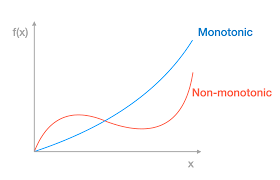
\includegraphics[width=0.5\textwidth]{assets/binary_search_on_the_answer/funcion_monotona_1.png}
	\end{figure}
\end{frame}

\begin{frame}{Funciones monótonas}
	\begin{TheoremP}[title=Función monotonamente decreciente]
		Sea f una función tal que $f: \mathbb{R} \rightarrow \mathbb{R}$. Se dice que f es monótonamente decreciente si para toda
		$x, y \in \mathbb{R}$ tal que $x < y$ tenemos que $f(x) \geq f(y)$
	\end{TheoremP}

	\begin{figure}[htbp]
		\centering
		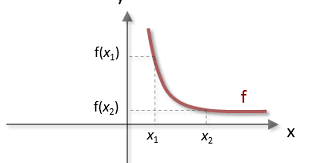
\includegraphics[width=0.5\textwidth]{assets/binary_search_on_the_answer/funcion_monotona_2.png}
	\end{figure}
\end{frame}

\begin{frame}{Busqueda binaria sobre la respuesta}
	Si tenemos un dominio o intervalo de posibles valores en los que se puede encontrar nuestra respuesta,
	entonces podemos hacer busqueda binaria para encontrarla, pero solo si nuestro espacio de busqueda tiene la forma
	de una función monótona.

	\vspace{0.5cm}

	Cada vez que saquemos la mitad de nuestro intervalo, digamos que es el valor $m$, vamos a pobrar si dicha posible respuesta $m$
	soluciona nuestro problema, y dependiendo de si lo hace o no, reducimos nuestro espacio de busqueda a la derecha o a la izquierda.
\end{frame}

\begin{frame}{Problema de práctica}
	\begin{itemize}
		\practiceproblem{Books}{Easy}{Codeforces}{https://codeforces.com/problemset/problem/279/B}
	\end{itemize}
\end{frame}
